\documentclass[letterpaper,10pt,twocolumn,twoside,]{pinp}

%% Some pieces required from the pandoc template
\providecommand{\tightlist}{%
  \setlength{\itemsep}{0pt}\setlength{\parskip}{0pt}}

% Use the lineno option to display guide line numbers if required.
% Note that the use of elements such as single-column equations
% may affect the guide line number alignment.

\usepackage[T1]{fontenc}
\usepackage[utf8]{inputenc}

% pinp change: the geometry package layout settings need to be set here, not in pinp.cls
\geometry{layoutsize={0.95588\paperwidth,0.98864\paperheight},%
  layouthoffset=0.02206\paperwidth, layoutvoffset=0.00568\paperheight}

\definecolor{pinpblue}{HTML}{185FAF}  % imagecolorpicker on blue for new R logo
\definecolor{pnasbluetext}{RGB}{101,0,0} %



\title{Neighbourhood Conditions on Boston Housing Value}

\author[a]{Matthew Shu}
\author[a]{Monica Turkovic}
\author[a]{Raissa Putrizulfan}
\author[a]{Yonatan Oron}
\author[a]{Ethan Hirschowitz}

  \affil[a]{University of Sydney}

\setcounter{secnumdepth}{0}

% Please give the surname of the lead author for the running footer
\leadauthor{}

% Keywords are not mandatory, but authors are strongly encouraged to provide them. If provided, please include two to five keywords, separated by the pipe symbol, e.g:
 

\begin{abstract}
The aim of this study was to construct a multiple linear regression
model on Boston Metropolitan Area housing value, based on the dataset
published by Harrison and Rubinfeld (1978), and evaluate the impact of
the neighbourhood characteristics. Optimising BIC lead to a parsimonious
model of 10 regressors (\(BIC=-710\), \(CV: R^2 = 0.78\)). It was found
that neighbourhood factors had a significant impact with the proportion
of the population at a low socioeconomic status having a large effect.
Limitations and areas of future research are discussed below.
\end{abstract}

\dates{This version was compiled on \today} 


% initially we use doi so keep for backwards compatibility
% new name is doi_footer
\doifooter{Neighbourhood Conditions on Boston Housing Value}

\pinpfootercontents{DATA2002}

\begin{document}

% Optional adjustment to line up main text (after abstract) of first page with line numbers, when using both lineno and twocolumn options.
% You should only change this length when you've finalised the article contents.
\verticaladjustment{-2pt}

\maketitle
\thispagestyle{firststyle}
\ifthenelse{\boolean{shortarticle}}{\ifthenelse{\boolean{singlecolumn}}{\abscontentformatted}{\abscontent}}{}

% If your first paragraph (i.e. with the \dropcap) contains a list environment (quote, quotation, theorem, definition, enumerate, itemize...), the line after the list may have some extra indentation. If this is the case, add \parshape=0 to the end of the list environment.

\acknow{This template package builds upon, and extends, the work of the
excellent \href{https://cran.r-project.org/package=rticles}{rticles}
package, and both packages rely on the
\href{http://www.pnas.org/site/authors/latex.xhtml}{PNAS LaTeX} macros.
Both these sources are gratefully acknowledged as this work would not
have been possible without them. Our extensions are under the same
respective licensing term
(\href{https://www.gnu.org/licenses/gpl-3.0.en.html}{GPL-3} and
\href{https://www.latex-project.org/lppl/}{LPPL (\textgreater= 1.3)}).}

\hypertarget{introduction}{%
\subsection{Introduction}\label{introduction}}

Hedonic Price Modelling has been a valuable method to estimate market
prices based on associated characteristics separate from the market
\citep{HARRISON197881, GOODMAN1978471} {[}1,14{]}. Accurately predicted
outcomes are valuable for many industries, including homeowners'
insurance, mortgages, price index construction, mass appraisal, and
other econometric studies of housing markets {[}13{]}. In one study of
hedonic house pricing by Harrison and Rubinfeld (1978), the 1970 census
data from the Boston Metropolitan Area was used to find willingness to
pay for better air quality. In this study, the same dataset will be used
to answer two important questions; (i) what is the predictive power of
this hedonic housing price model on housing prices (ii) how does the
neighbourhood conditions of an area affect housing value.

\hypertarget{dataset}{%
\subsection{Dataset}\label{dataset}}

\hypertarget{analysis}{%
\subsection{Analysis}\label{analysis}}

Prior to further analysis, the assumptions of linearity, independence,
homoscedasticity and normality were checked for the full model. Due to
poor linearity within pairwise plots, various transformations were
considered. The extreme skew of ZN, B and RAD made them good candidates
for individual log transformation. However, it was found that the
residuals vs.~fitted plot linearity was only fulfilled with a further
log transformation of the MEDV i.e.~a log-log relationship. The
log-transformed outcome is displayed in the residuals-fitted plot in
Figure \ref{fig:partial_log_full_lm_residuals}, where the approximately
levelled line indicates a good fit of linearity. As this dataset was
collected from the 1970 U.S Census and various governmental
organisations, it is presumed that the design of the experiment produced
observations that were independent of each other. However, the plausible
spatial dependency between house values within the Boston Metropolitan
area is perhaps a limitation in the independence assumption. Thirdly,
while a slight fanning-in in the log-transformed residuals-fitted plot
is observed, there is an approximately constant spread over the range of
fitted values, indicating homoscedasticity. Finally, as in Figure
\ref{fig:partial_log_full_lm_qq} observations in the QQ plot appear to
deviate in the extremities, however, the Central Limit Theorem can be
applied to satisfy the normality assumption due to the large set of
observations in the data set.

\hypertarget{refined-model}{%
\subsection{Refined Model}\label{refined-model}}

To refine the model, a Bayesian Information Criterion (BIC) was used,
which appropriately punishes the use of excessive regressors {[}5{]}.
This was applied to both an exhaustive, backwards and forwards search to
assess the efficacy of models of different sizes and explanatory
variables. All three searches, minimising BIC, are in agreement that a
model size of 10 regressors omitting AGE, INDUS and ZN provides an
appropriate balance between in-sample predictive power and the number of
regressors.

The residuals-fitted plot indicates the linearity assumption is
fulfilled with slight overestimates near the extremities as in Fig
\ref{fig:refined_lm_residuals}. The residuals also appear to be
homoscedastic with only slight fanning. The QQ-plot indicates residuals
appear mostly normal with a slight deviation near the extremities as in
Fig \ref{fig:refined_lm_qq}. Given 506 samples, the test statistic can
still be assumed to follow the expected distribution by appealing to the
Central Limit Theorem.

The refined model was subsequently checked for multicollinearity by
assessing the Variance Inflation Factor. All variables had a VIF
\textless{} 10 indicating multicollinearity is not a major issue for the
refined model {[}6{]}.

You can get model coefficients from Main.Rmd in Model Refinement
section. Please include an equation for us.

\begin{equation}
  \begin{aligned}
(x+y)^3&=(x+y)(x+y)^2\\
       &=(x+y)(x^2+2xy+y^2) \\
       &=x^3+3x^2y+3xy^3+x^3. 
       \label{eqn:example} 
  \end{aligned}
\end{equation}

\hypertarget{results}{%
\subsection{Results}\label{results}}

\hypertarget{cross-validation}{%
\subsubsection{Cross Validation}\label{cross-validation}}

A 100-repeated 10-fold cross-validation was then performed on both the
full model and refined model to assess the out-of-sample performance
between models. Extremely similar R\^{}2 values of approximately 0.78
indicated that the refined model with fewer regressors did not sacrifice
much in the way of predictive power. In the interest of parsimony, the
refined model was chosen. (Graph of R2/MAE if able to fit)

\hypertarget{model-interpretation}{%
\subsubsection{Model Interpretation}\label{model-interpretation}}

Cohen's f\^{}2 score was used to determine the effect size of individual
predictors in the refined multiple regression model {[}7{]}. Based on
standard cut-offs, LSTAT was found to have a large effect size whilst
all other regressors had small or negligible effect size {[}D{]}.

We have decided to focus primarily on four neighbourhood variables in
our problem statement. namely LSTAT, CRIM, PTRATIO and CHAS. Past
research has concluded that there is a positive relationship between
household income and property values {[}8{]}. This was greatly reflected
in our data, where Cohen's f\^{}2 analysis found that LSTAT had the
greatest effect on housing prices, as a one unit increase in the
proportion of ``lower status'' individuals in the area corresponds to a
2.9\% decrease in median house value. It has been well known that crime
decreases the overall value of a property. In our model we see that a
one unit increase in crime rate will result in a 1\% decrease in median
house value. Past research has reported that school accessibility
{[}10{]} and quality {[}11{]} has a positive effect on the value of
property surrounding it, where the closer a house is from a school, the
higher its price. Our model states that a one unit increase in PTRATIO
corresponds to a 4\% decrease in house prices. Interestingly this is in
disagreement with past literature by Aliyu (2016), Seo and Simons
(2009). Past research has indicated that waterfront properties mostly
sell at a higher price {[}12{]}. This was reflected in our model where a
one unit increase in house price corresponds with a 10.5\% increase in
CHAS.

\hypertarget{discussion}{%
\subsection{Discussion}\label{discussion}}

When analysing the dataset, different contextual limitations of the data
were encountered. These limitations were mostly related to the
irrelevance of Boston data from the 1970's to modern housing markets. It
was noticeable that many of the predictor variables used would have
little impact on housing prices today due to shifts in societal
perspectives and attitudes. For example, the B variable (proportion of
blacks) would be an outdated and irrelevant metric in modern housing
markets. Other factors such as inflation and changes in the volatilities
of housing markets also meant that adjustments would have to be made to
the model.

Another major issue was multicollinearity amongst the independent
variables. Since the independent variables could be classified into
categories such as neighbourhood, pollution and accessibility, there was
concern that variables in the same category may be highly
intercorrelated. Replicating the approach of the study from which the
dataset was sourced, a VIF multicollinearity check was used to ensure
that the independent variables had sufficiently low
intercorrelation{[}1{]}.

In the final model, one of the most significant independent variables
was the crime rate (CRIM). There was concern that the crime rate was too
general a predictor, since it was expected that different types of
crimes would have differing impacts on house prices. Specifically,
impacts of violent crime versus ``white collar'' crime. An article on
the Australian housing market found that many major Australian cities
were experiencing simultaneous increases in housing prices and crime
rates {[}2{]}. Whilst this does not necessarily mean that the two are
correlated, it does indicate that in modern days, society may perhaps
place more value on location and accessibility over perceived safety. A
different study on the relationship between levels of crime and housing
prices found that rather than actual crime rates, proximity to crime
hotspots had a more significant impact on house prices {[}3{]}. Results
showed that specific types of crimes had different effects on the
housing market. It was found that the crime with the most significant
impact on house prices was vandalism, indicating that housing markets
are potentially most concerned about crimes that affect the physical
appearance of a neighbourhood.

Based on the findings, it is possible to make recommendations for future
research on similar datasets. It is important to ensure that independent
variables are contextually relevant and reflective of the general
population, by using recent data from a large sample size. Additionally,
it is vital to minimise multicollinearity in the model. This could be
done by ensuring that independent variables are not intercorrelated by
selecting predictors from different sources and fields. Lastly,
variables should be adjusted to ensure that they accurately measure the
impact on the dependent variable. For example, future studies on the
impacts of different factors on house prices could consider proximity to
crime hotspots or levels of vandalism rather than the general crime
rate.

\hypertarget{conclusion}{%
\subsection{Conclusion}\label{conclusion}}

Overall, the regression model was successful in modelling different
impacts on housing prices in Boston in the 1970's. Research found that
variables such as crime rate, social status of the population and the
ratio of pupils to teachers, all belonging to the general group of
``quality of the neighbourhood'' had the largest impact on house prices.
Whilst the model was able to predict house prices for that specific
housing market, due to the obsolescence of the data, it would be
impossible to predict modern house prices.

\hypertarget{appendix}{%
\subsection{Appendix}\label{appendix}}

INSERT DATA DESCRIPTION TABLE

\begin{figure}[!H]

{\centering \includegraphics{Final_Report_files/figure-latex/partial_log_full_lm_residuals-1} 

}

\caption{\label{fig:partial_log_full_lm_residuals}Residuals plot against fitted values of full model after log transformation.}\label{fig:partial_log_full_lm_residuals}
\end{figure}

\begin{figure}

{\centering \includegraphics{Final_Report_files/figure-latex/partial_log_full_lm_qq-1} 

}

\caption{\label{fig:partial_log_full_lm_qq}QQ plot of full model residuals after log transformation.}\label{fig:partial_log_full_lm_qq}
\end{figure}

\begin{figure}

{\centering \includegraphics{Final_Report_files/figure-latex/refined_lm_residuals-1} 

}

\caption{\label{fig:refined_lm_residuals}Residuals plot against fitted values of refined model. Slight difference.}\label{fig:refined_lm_residuals}
\end{figure}

\begin{figure}

{\centering \includegraphics{Final_Report_files/figure-latex/refined_lm_qq-1} 

}

\caption{\label{fig:refined_lm_qq}QQ plot of refined model residuals. Slight difference.}\label{fig:refined_lm_qq}
\end{figure}

\hypertarget{original-template}{%
\subsection{Original Template}\label{original-template}}

\textbf{Everything underneath is a template that helps direct how to add
various objects to the report.}

This \emph{pinp is not PNAS} template started when the introduction to
\href{http://dirk.eddelbuettel.com/code/rcpp.html}{Rcpp} by
\cite{PeerJ:Rcpp} was converted into this updated
\href{https://eddelbuettel.github.io/pinp/Rcpp-introduction.pdf}{Rcpp
Introduction} vignette. It is based on the
\href{https://github.com/rstudio/rticles/tree/master/inst/rmarkdown/templates/pnas_article}{pnas\_article}
template of the wonderful
\href{https://cran.r-project.org/package=rticles}{rticles} package by
\cite{CRAN:rticles}. The conversion from markdown to latex is
facilitated by
\href{https://cran.r-project.org/package=rmarkdown}{rmarkdown}
\citep{CRAN:rmarkdown} and
\href{https://cran.r-project.org/package=knitr}{knitr}
\citep{CRAN:knitr}. The underlying LaTeX macros are from
\href{http://www.pnas.org/site/authors/latex.xhtml}{pnas.org}.

The remainder of the document carries over from the corresponding
\href{https://github.com/rstudio/rticles/tree/master/inst/rmarkdown/templates/pnas_article}{pnas\_article}
template document. but has been edited and updated to our use case. A
few specific tips follow. In general, for fine-tuning some knowledge of
LaTeX is helpful.

\hypertarget{author-affiliations}{%
\subsection{Author Affiliations}\label{author-affiliations}}

Per common academic best practice, you can include your department,
institution, and complete address, with the ZIP/postal code, for each
author. Use lower case letters to match authors with institutions, as
shown in the example. Authors with an ORCID ID may supply this
information at submission.

\hypertarget{document-options}{%
\subsection{Document Options}\label{document-options}}

We support several options via the YAML header

\begin{itemize}
\tightlist
\item
  Setting a DOI or URL footer, for example for the CRAN package URL,
  which is placed in the bottom-left footer of the title page and even
  pages;
\item
  Setting a footer label, for example \emph{YourPackage Vignette}
  stating your package, which is placed in the bottom-right footer on
  odd pages;
\item
  Setting a free-form author field used on the inside footer;
\item
  Optional \emph{Draft} watermark to be added to each page;
\item
  Line of custom text in subtitle (\texttt{date\_subtitle}) suitable to
  give publication info of the draft, e.g.~journal name in a post-print;
\item
  Document date that appears in the footer can be specified manually
  using \texttt{document\_date}.
\end{itemize}

\hypertarget{references}{%
\subsection{References}\label{references}}

Here we differ from PNAS and suggest natbib. References will appear in
author-year form. Use \texttt{\textbackslash{}citet\{\}},
\texttt{\textbackslash{}citep\{\}}, etc as usual.

We default to the \texttt{jss.bst} style. To switch to a different
bibliography style, please use \texttt{biblio-style:\ style} in the YAML
header.

\hypertarget{inline-r-code}{%
\subsection{Inline R Code}\label{inline-r-code}}

The PNAS sample included a fixed PNG image here, but this document
prefers to show the results and embedding of \emph{R} code.

\begin{Shaded}
\begin{Highlighting}[]
\FunctionTok{library}\NormalTok{(ggplot2)}
\FunctionTok{ggplot}\NormalTok{(mtcars, }\FunctionTok{aes}\NormalTok{(wt, mpg)) }\SpecialCharTok{+}
    \FunctionTok{geom\_point}\NormalTok{(}\AttributeTok{size=}\DecValTok{3}\NormalTok{, }\FunctionTok{aes}\NormalTok{(}\AttributeTok{colour=}\FunctionTok{factor}\NormalTok{(cyl))) }\SpecialCharTok{+}
    \FunctionTok{theme}\NormalTok{(}\AttributeTok{legend.position=}\StringTok{"none"}\NormalTok{)}
\end{Highlighting}
\end{Shaded}

\begin{figure}

{\centering \includegraphics{Final_Report_files/figure-latex/figex-1} 

}

\caption{Narrow ggplot2 figure}\label{fig:figex}
\end{figure}

Here we use a standard knitr bloc with explicit options for

\begin{itemize}
\tightlist
\item
  figure width and height (\texttt{fig.width}, \texttt{fig.height}),
  both set to three inches;
\item
  whether the code is shown (\texttt{echo=TRUE}); and
\item
  the caption (\texttt{fig.cap}) as shown above.
\end{itemize}

\hypertarget{digital-figures}{%
\subsection{Digital Figures}\label{digital-figures}}

Markdown, Pandoc and LaTeX support \texttt{.eps} and \texttt{.pdf}
files.

Figures and Tables should be labelled and referenced in the standard way
using the \texttt{\textbackslash{}label\{\}} and
\texttt{\textbackslash{}ref\{\}} commands.

The R examples above show how to insert a column-wide figure. To insert
a figure wider than one column, please use the
\texttt{\textbackslash{}begin\{figure*\}...\textbackslash{}end\{figure*\}}
environment.

One (roundabout) way of doing this is to \emph{not} actually plot a
figure, but to save it in a file as the following segment shows:

\begin{Shaded}
\begin{Highlighting}[]
\FunctionTok{library}\NormalTok{(ggplot2)}
\NormalTok{p }\OtherTok{\textless{}{-}} \FunctionTok{ggplot}\NormalTok{(}\AttributeTok{data =}\NormalTok{ midwest,}
            \AttributeTok{mapping =} \FunctionTok{aes}\NormalTok{(}\AttributeTok{x =}\NormalTok{ area,}
                          \AttributeTok{fill =}\NormalTok{ state,}
                          \AttributeTok{color =}\NormalTok{ state)) }\SpecialCharTok{+}
    \FunctionTok{geom\_density}\NormalTok{(}\AttributeTok{alpha =} \FloatTok{0.3}\NormalTok{)}
\DocumentationTok{\#\# save to file}
\FunctionTok{suppressMessages}\NormalTok{(}\FunctionTok{ggsave}\NormalTok{(}\StringTok{"densities.pdf"}\NormalTok{, p))}
\end{Highlighting}
\end{Shaded}

This file is then included via standard LaTeX commands.

\begin{figure*}
  \begin{center}
    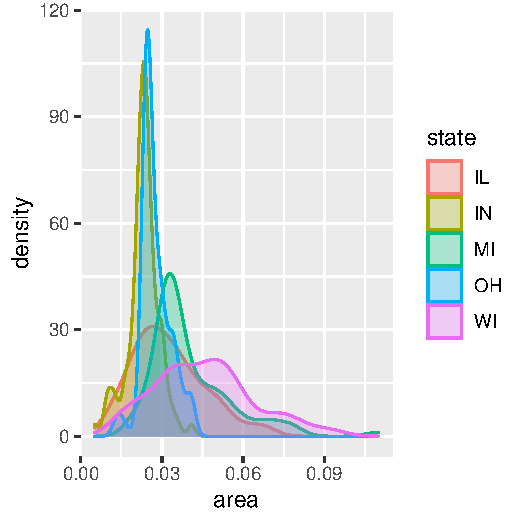
\includegraphics[width=0.66\textwidth, height=3.5in]{densities} 
  \end{center}
  \caption{Wide ggplot2 figure}\label{fig}
\end{figure*}

\hypertarget{typeset-code-but-do-not-run-it}{%
\subsection{Typeset Code (But Do Not Run
It)}\label{typeset-code-but-do-not-run-it}}

We can also just show code.

\begin{Shaded}
\begin{Highlighting}[]
\NormalTok{xx }\OtherTok{\textless{}{-}}\NormalTok{ faithful[,}\StringTok{"eruptions"}\NormalTok{]}
\NormalTok{fit }\OtherTok{\textless{}{-}} \FunctionTok{density}\NormalTok{(xx)}
\FunctionTok{plot}\NormalTok{(fit)}
\end{Highlighting}
\end{Shaded}

This simply used a pandoc bloc started and ended by three backticks,
with \texttt{r} as the language choice. Similarly, \emph{many} other
languages can be typeset directly simply by relying on pandoc.

\hypertarget{single-column-equations}{%
\subsection{Single column equations}\label{single-column-equations}}

Authors may use 1- or 2-column equations in their article, according to
their preference.

To allow an equation to span both columns, options are to use the
\texttt{\textbackslash{}begin\{figure*\}...\textbackslash{}end\{figure*\}}
environment mentioned above for figures. The
\texttt{\textbackslash{}begin\{widetext\}...\textbackslash{}end\{widetext\}}
environment as shown in equation \ref{eqn:example} below is deprecated,
but \LaTeX commands \texttt{\textbackslash{}onecolumn} and
\texttt{\textbackslash{}twocolumn} work fine.

Please note that this option may run into problems with floats and
footnotes, as mentioned in the \href{http://texdoc.net/pkg/cuted}{cuted
package documentation}. In the case of problems with footnotes, it may
be possible to correct the situation using commands
\texttt{\textbackslash{}footnotemark} and
\texttt{\textbackslash{}footnotetext}.

\begin{equation}
  \begin{aligned}
(x+y)^3&=(x+y)(x+y)^2\\
       &=(x+y)(x^2+2xy+y^2) \\
       &=x^3+3x^2y+3xy^3+x^3. 
       \label{eqn:example} 
  \end{aligned}
\end{equation}

%\showmatmethods
\showacknow


\bibliography{references}
\bibliographystyle{jss}



\end{document}
